% modified from the TUG example by: Jean-C\^ome Charpentier 2005
% Compile with XeLaTeX
\documentclass{article}

\usepackage[margin=0.5in]{geometry}
\usepackage{graphicx}
\usepackage{xcolor}
\usepackage{pstricks}

\begin{document}
\thispagestyle{empty}

\noindent
\begin{pspicture}(0,13.5)(\linewidth,0)
  \psline[linewidth=3mm,linecolor=black](0,13.5)(\linewidth,13.5)
  \rput(\linewidth,13.5)
    {\pspolygon*(-3.6,0)(-1.4,0)(0,-1.4)(0,-3.6)}
  \rput(\linewidth,13.5)
    {\rput{-45}(-1,-1){\Large\textbf{\white Version}}}
  \rput(\linewidth,13.5)
    {\rput{-45}(-1.5,-1.5){\Large\textbf{\white 1.1}}}

	\rput[b]{4}(9.5,-2.7){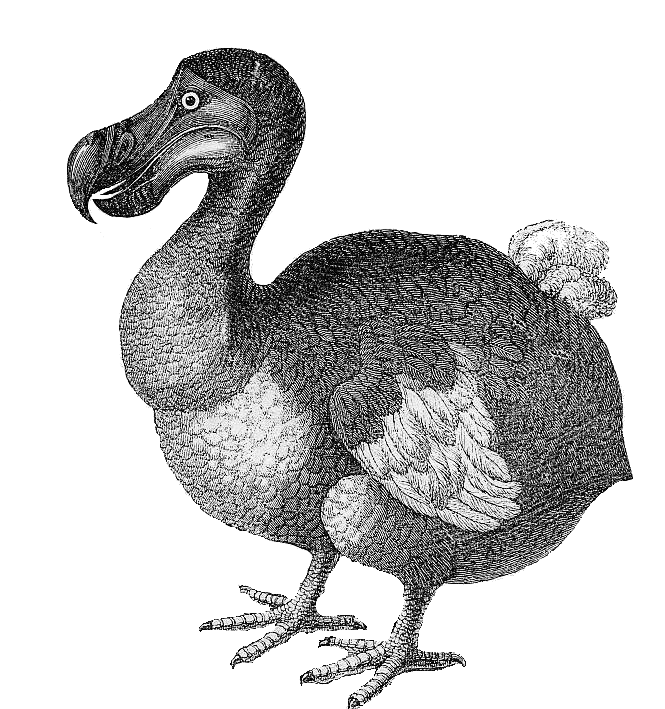
\includegraphics[scale=1.4]{DODO1.png}}
    
  \psline[linewidth=2mm,linecolor=black](0,-3)(\linewidth,-3)
  \rput[l](0,-4.5){\psscaleboxto(\textwidth,2){Guide to the \textbf{memuse} Package}}
  \psline[linewidth=2mm,linecolor=black](0,-6)(\linewidth,-6)
  \rput[l](0,-6.8){\textsl{\huge A Package for Estimating Memory Usage}}
  \end{pspicture}

\vfill\noindent
\ \hfill {\large\textsl{Drew Schmidt}}
\end{document}
